
\chapter{Giới thiệu chung} 
\minitoc
\vspace{0.5cm}
\noindent
% Trong chương này, ta xem xét phạm vi của khoa học máy tính, lịch sử phát triển và các kiến
% thức nền tảng chuẩn bị cho các chương tiếp theo.
Khoa học máy tính là một chuyên ngành nhằm xây dựng cơ sở khoa học cho những lĩnh vực như
thiết kế máy tính, lập trình, xử lý thông tin, thuật toán, giải quyết vấn đề dựa
trên thuật toán, và cả quá trình xây dựng thuật toán. Nó cung cấp nền tảng cho các ứng
dụng tin học hiện tại cũng như tương lai.

%Cuốn sách này nhằm giới thiệu một cách tổng quan về khoa học máy tính. Tuy nhiên, ta cũng muốn đánh
%giá đầy đủ phạm vi và tính động của ngành học này; vì vậy, ngoài các chủ đề nghiên cứu
%chính, ta còn xem xét đến lịch sử phát triển, hiện trạng, và những hướng nghiên cứu trong tương lai. Mục tiêu của cuốn sách là giúp người đọc hiểu về các chức
%năng của khoa học máy tính--những kiến thức này không những có ích cho những người làm
%nghiên cứu mà còn cho cả những người làm trong lĩnh vực ứng dụng công nghệ.
 

\section{Vai trò của thuật toán}

Ta bắt đầu với khái niệm cơ bản nhất của khoa học máy tính--khái niệm thuật toán. Hiểu nôm
na, một \textbf{thuật toán} là một dãy các bước xác định cách thực hiện một nhiệm vụ nào
đó.  (Ta sẽ định nghĩa một cách chính xác hơn trong Chương \ref{}.) Ví dụ, thuật toán
để nấu ăn (gọi là công thức nấu ăn), thuật toán để tìm đường (hay còn gọi là chỉ đường),
thuật toán để vận hành máy giặt (thường được ghi bên trong nắp của máy giặt hoặc trên
tường của hiệu giặt tự động), thuật toán để chơi nhạc (thể hiện dưới dạng các bản
nhạc)...

% \begin{comment}
% \begin{figure}
%   \begin{quotation}
%     \noindent
%     \textbf{Luật chơi:} Nhà ảo thuật lấy vài quân bài từ bộ bài chuẩn đặt úp xuống bàn và
%     tráo chúng cẩn thận trước khi trải chúng lên bàn. Sau đó người chơi được yêu cầu lấy
%     các quân bài hoặc quân đỏ, hoặc quân đen, và nhà ảo thuật sẽ lật quân bài đúng màu
%     được yêu cầu.

%     \vspace{0.5cm}
%     \noindent
%     \textbf{Làm ra vẻ bí mật và nói một cách máy móc theo chỉ dẫn dưới đây:}
%     \begin{description}
%     \item[Bước 1] Từ bộ bài chuẩn, chọn muời cây đỏ và mười cây đen. Đặt các quân bài này
%       ngửa lên thành hai cột theo màu.

%     \item[Bước 2] Thông báo rằng bạn sẽ chọn một vài quân đỏ và một vài quân đen.

%     \item[Bước 3] Chọn các quân bài đỏ. Giả vờ xếp chúng vào trong bộ bài nhỏ, nhưng thực
%       ra vẫn giữ chúng úp mặt trong tay trái và, với ngón tay cái và ngón trỏ của bàn tay
%       phải, kéo quân cuối cùng của bộ bài lên sao cho mỗi quân bị bẻ hơi cong về
%       \textit{phía sau}. Sau đó đặt quân bài màu đỏ xuống bàn và nói, ``Đây là quân đỏ đã
%       được bố trí trước trong bộ bài.''

%     \item[Bước 4] Chọn các quân đen. Theo cách tương tự như bước 3, đưa các quân này về
%       \textit{phía trước}. Sau đó đưa trả quân bài này về bàn và nói, ``Và đây là quân bài
%       màu đen đã được bố trí trước.''

%     \item[Bước 5] Ngay sau khi trả quân bài đen trở lại bàn, cả hai tay trộn quân bài màu
%       đen (vẫn úp) như bạn căng ra trên bàn. Giải thích rằng bạn đang trộn cẩn thận các
%       quân bài.

%     \item[Bước 6] Trong khi bỏ quân bài xuống bàn, lặp lại các bước sau đây:
%       \begin{enumerate}
%       \item Hỏi người chơi xem yêu cầu quân đỏ hay quân đen.

%       \item Nếu màu được yêu cầu là màu đỏ và có một vết lõm xuất hiện trên quân bài đặt
%         xuống, lật quân bài lên và nói, ``Đây là quân đỏ''.

%       \item Nếu quân bài được yêu cầu là màu đen và có một vết lõm trên quân bài đặt
%         xuống, lật quân bài và nói ``Đây là quân đen''.

%       \item Ngược lại, khẳng định rằng không còn quân bài nào có màu được yêu cầu và đặt
%         các quân bài còn lại xuống bàn và lật lên để chứng minh khẳng định của mình.
%       \end{enumerate}
%     \end{description}
%   \end{quotation}
%   \caption{Một thuật toán cho một magic trick}
%   \label{fig:fig0.1}
% \end{figure}
% \end{comment}

Trước khi một máy (kiểu như máy tính) có thể thực hiện một nhiệm vụ nào đó, ta phải tìm ra
một thuật toán để thực hiện nhiệm vụ đó và biểu diễn nó dưới dạng thích hợp với máy. Một
biểu diễn của một thuật toán được gọi là một \textbf{chương trình}. Để thuận tiện cho con
người, các chương trình  thường được in trên giấy hoặc hiển thị trên màn hình máy
tính. Để thuận tiện cho máy, các chương trình được mã hóa thích hợp với công
nghệ của máy. Quá trình phát triển một chương trình, mã hóa nó dưới dạng thích hợp, và đưa nó vào máy tính được gọi là \textbf{lập trình}. Chương trình và các thuật
toán mà nó biểu diễn được gọi chung là \textbf{phần mềm}; còn máy được gọi là
\textbf{phần cứng}.

Ban đầu việc nghiên cứu về thuật toán được xem là một nghành thuần túy toán học.  Các nhà toán học đã nghiên cứu thuật toán từ rất lâu trước khi có sự xuất hiện của máy tính. Mục tiêu của họ
là tìm ra một tập các chỉ dẫn để mô tả hướng giải quyết của một lớp bài toán thuộc cùng
một dạng đặc biệt. Một ví dụ nổi tiếng  là
thuật toán chia để tìm thương của hai số có nhiều chữ số. Một ví dụ khác là thuật toán
Euclid, được tìm thấy bởi nhà toán học cổ Hy Lạp Euclid, để tìm ước chung nhỏ lớn nhất của
hai số nguyên~(Hình~\ref{fig:fig0.2}).

Sau khi đã tìm được một thuật toán thực hiện một nhiệm vụ cho trước, ta có thể thực hiện
nhiệm vụ này mà không cần phải hiểu thuật toán đó dựa trên nguyên lý gì. Việc thực hiện
nhiệm vụ bây giờ chỉ đơn giản là làm đi theo các chỉ dẫn. Ví dụ, ta có thể
thực hiện thuật toán chia để tìm thương hoặc thuật toán Euclid để tìm ước chung lớn nhất mà
không cần hiểu tại sao lại làm được như vậy.  Theo một nghĩa nào đó, trí tuệ cần thiết để
giải các bài toán này đã được mã hoá dưới dạng thuật toán.



\begin{figure}[tb]
  \begin{quotation}
    \noindent
    \textbf{Mô tả:} Thuật toán thực hiện tính ước chung lớn nhất của hai số
    nguyên dương.

    \vspace{0.5cm}
    \noindent
    \textbf{Thủ tục:}
    \begin{description}
    \item[Bước 1] Với hai số đầu vào, ta gán số lớn cho $M$ và số nhỏ cho $N$.

    \item[Bước 2] Chia $M$ cho $N$, và đặt phần dư là $R$.

    \item[Bước 3] Nếu $R$ khác $0$ thì gán $M$ bằng giá trị của $N$, gán lại~$N$
      bằng giá trị của~$R$, và quay trở lại bước $2$; ngược lại, ước chung lớn
      nhất chính là giá trị hiện thời của  $N$.
    \end{description}
  \end{quotation}
  \caption{Thuật toán Euclid để tìm ước chung lớn nhất của hai số nguyên dương}
  \label{fig:fig0.2}
\end{figure}


Nhờ việc ta có thể truyền tải trí thông minh dưới dạng thuật toán mà ta có thể tạo nên các
máy thực hiện các nhiệm vụ mà ta mong muốn. Và mức độ thông minh của máy
sẽ chỉ giới hạn trong việc những trí thông minh có thể truyền tải thành thuật toán. Ta chỉ
có thể xây dựng một máy để thực hiện một nhiệm vụ nếu tồn tại một thuật toán để thực hiện
nhiệm vụ đó. Ngược lại, nếu không có thuật toán để giải một bài toán thì việc giải quyết
bài toán này nằm ngoài khả năng của máy.


Việc phát hiện ra giới hạn của phương pháp thuật toán đã trở thành một chủ đề của toán học
từ những năm 1930 với công trình của Kurt G\"odel về định lý không toàn vẹn
(incompleteness theorem). Định lý này về cơ bản khẳng định rằng trong mọi lý thuyết toán
học có chứa số học các số tự nhiên, có tồn tại những khẳng định mà việc quyết định nó đúng
hay sai không thể được xác định theo nghĩa của thuật toán. Nói một cách ngắn gọn, mọi nghiên cứu
đầy đủ  về hệ thống số học nằm ngoài khả năng của các hoạt động thuật toán.

Phát hiện này đã làm lung lay cơ sở toán học. Người ta đã bắt đầu một lĩnh vực mới gọi là
khoa học máy tính, chuyên nghiên cứu khả năng của phương pháp thuật toán.



%%% Local Variables: 
%%% mode: latex
%%% TeX-master: "../tindaicuong"
%%% End: 

\section{Lịch sử máy tính} 


Máy tính ngày nay có một phả hệ hết sức rộng rãi. Một trong những thiết bị tính toán ra
đời sớm nhất là bàn tính, được biết đến từ thời La Mã và Hy Lạp cổ đại. Máy này khá đơn
giản, bao gồm các hạt tròn được xâu lần lượt trên các que gắn trong một khung chữ nhật
(Hình \ref{fig:fig0.3}). Các hạt này có thể di chuyển qua lại trên các que, và các vị trí
của chúng thể hiện các giá trị lưu trữ. Vậy ``máy tính'' này biểu diễn và lưu trữ dữ liệu
chính trong các vị trí của các hạt này. Để điều khiển việc thực hiện thuật toán, máy phải
dựa vào người thao tác. Bởi vậy bản thân bàn tính chỉ đóng vai trò lưu trữ dữ liệu; nó
phải kết hợp với hoạt động của con người để tạo ra một máy hoàn chỉnh có thể tính toán
được.


\begin{figure}[tb]
\centering
    \scalebox{0.4}{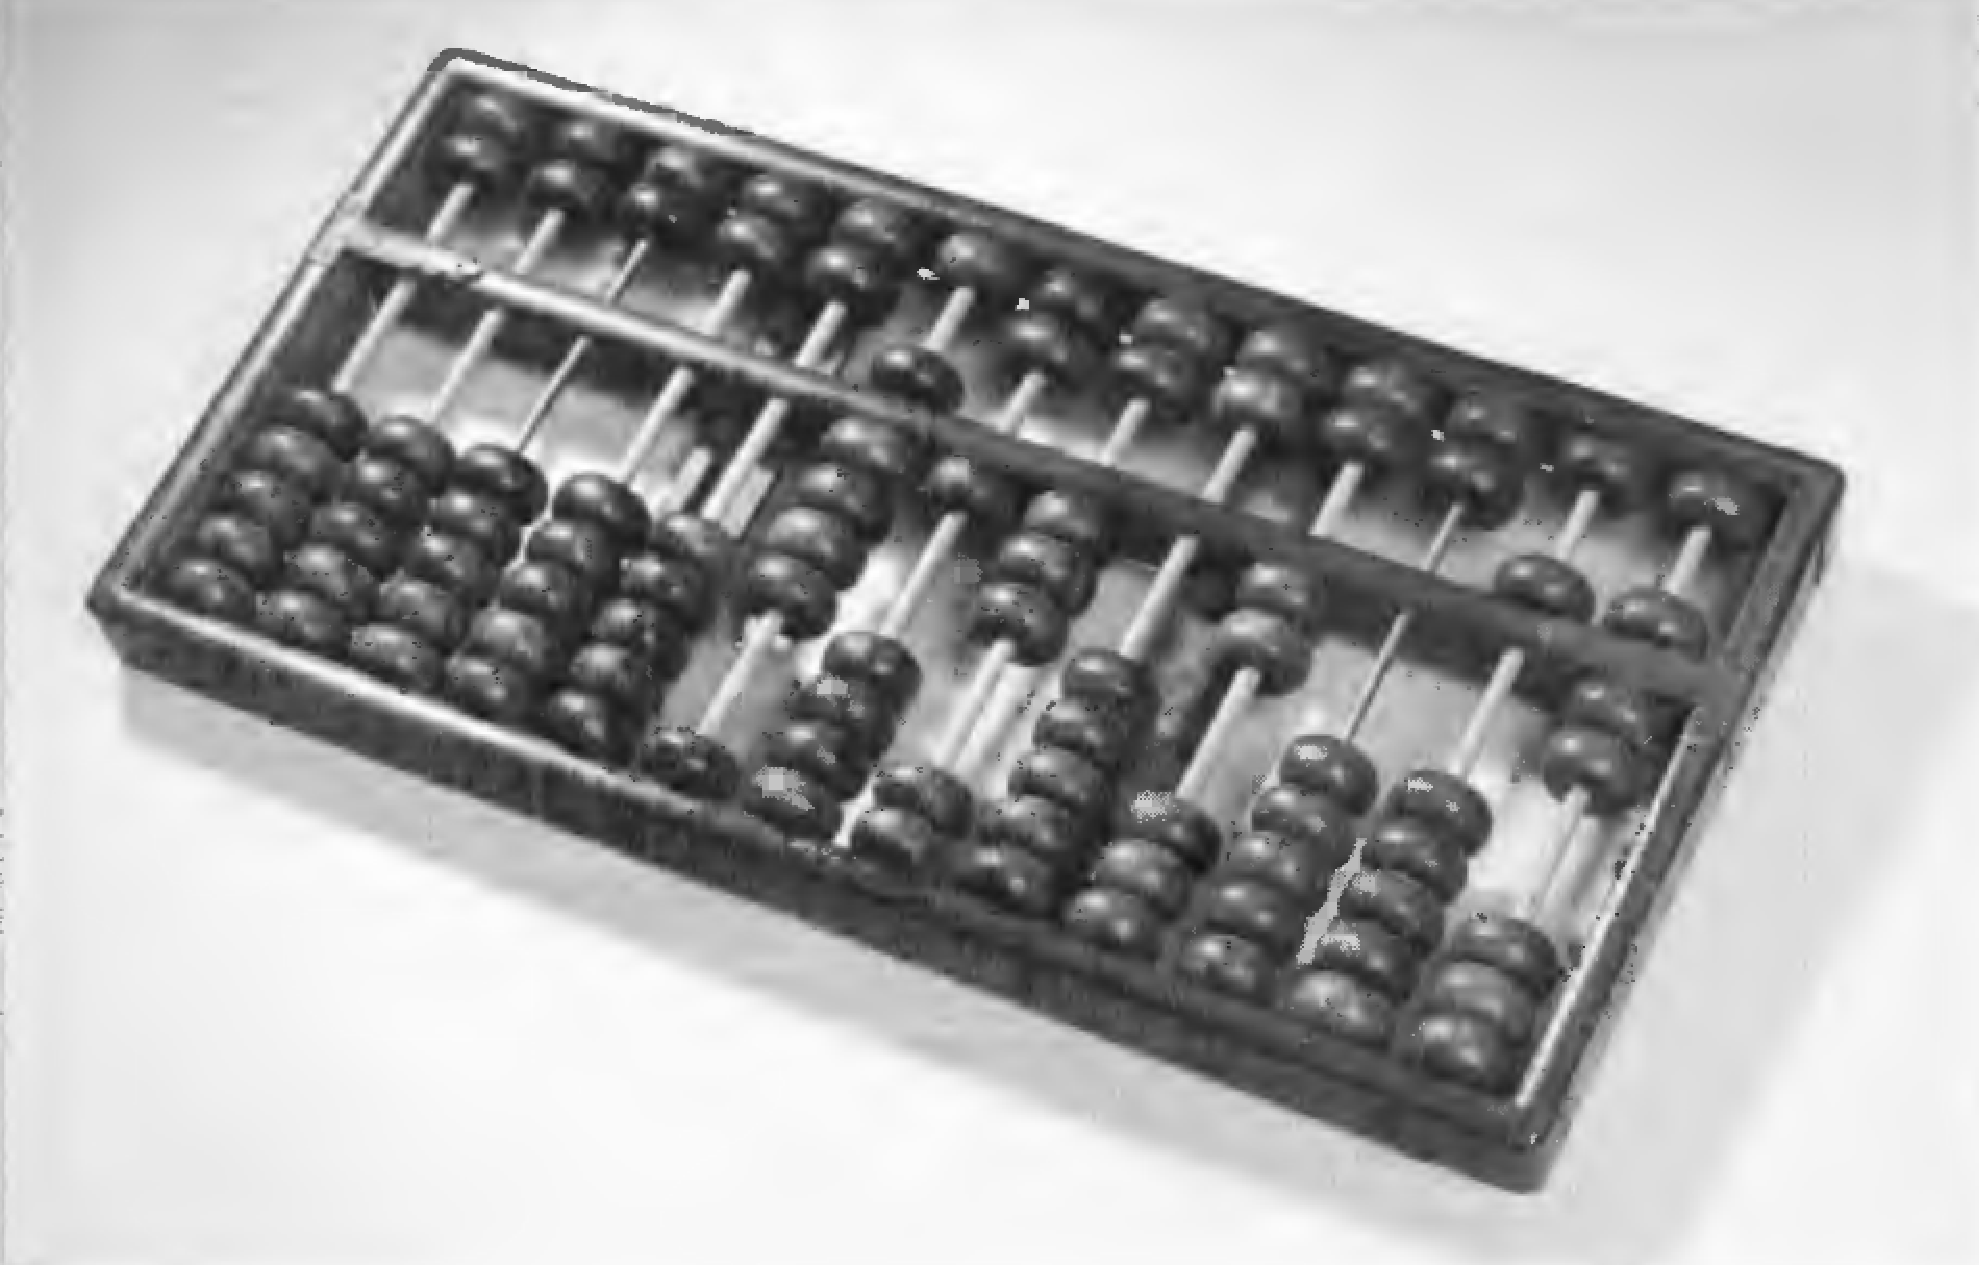
\includegraphics{ch0/fig03.pdf}}
\caption{Một bàn tính (ảnh chụp bởi Wayne Chandler)}
  \label{fig:fig0.3}
\end{figure}
 


Gần đây hơn, các thiết kế của máy tính đã dựa trên công nghệ cơ học. Một số nhà phát minh
trong thời kỳ này là Blaise Pascal (1623-1662) của Pháp, Wilhelm Gottfried Leibniz
(1646-1716) của Đức, và Charles Babbage (1792-1871) của Anh. Những máy này biểu diễn dữ
liệu thông qua vị trí của bánh răng, với các dữ liệu đầu vào được đặt một cách cơ học bằng
vị trí ban đầu của bánh răng.  Đầu ra của các máy của Pascal và của Leibniz đã được xác
định bằng cách quan sát các vị trí của bánh răng khi việc thực hiện kết thúc. Để tránh các sai sót khi ghi lại kết quả tính toán, 
Babbage đã thiết kế máy cho phép in luôn kết quả tính toán ra giấy.


Ta có thể thấy các máy ngày càng linh hoạt hơn (theo nghĩa làm việc theo thuật toán). Máy
của Pascal chỉ thực hiện phép cộng đơn giản bằng cách đặt một dãy các bước thích hợp ngay
trong bản thân cấu trúc của máy. Tương tự, máy của Leibniz có thuật toán được nhúng sẵn
vào trong kiến trúc của nó, mặc dù nó đã cho phép người dùng thao tác để lựa chọn trong
nhiều phép toán số học. Máy tính sai phân của Babbage (Babbage's Difference Engine), thực
ra nó vẫn chỉ là mô hình trên giấy, có thể thay đổi thực hiện nhiều phép toán phong phú;
và máy Phân tích (Analytical Engine), máy mà Babbage chưa bao giờ nhận được tài trợ để
làm, đã được thiết kế để đọc các lệnh dưới dạng các lỗ trên thẻ giấy. Bởi vậy máy Phân
tích của Babbage là có thể lập trình được. Trên thực tế, Augusta Ada Byron (Ada Lovelace)
đã xuất bản một bài báo chỉ ra cách lập trình trên máy Phân tích để thực hiện nhiều tính
toán. Và ngày nay người ta vẫn xem Ada như lập trình viên đầu tiên trên thế giới.


Ý tưởng biểu diễn các thuật toán thông qua giấy đục lỗ không phải bắt đầu từ Babbage. Ông
đã dựa trên ý tưởng trước đó của Joseph~Jacquard (1752-1834). Vào năm 1801,
Joseph Jacquard đã tạo nên một khung dệt, mà trong đó từng bước của quá trình dệt đã được
xác định bởi các mẫu lỗ đục trên thẻ giấy. Theo cách này, các thuật toán được thực hiện
bởi các khung dệt có thể thay đổi một cách dễ dàng theo các thiết kế mẫu dệt khác
nhau. Herman Hollerith (1860-1929) cũng đã sử dụng ý tưởng của Jacquard để tăng tốc độ xử
lý các bảng tính trong điều tra số dân của Mỹ năm 1890. Kiểu thẻ này sau đó đã được gọi là
thẻ đục lỗ đã là một phương tiện giao tiếp với máy tính rất phổ biến vào những năm
1970s. Cho đến nay các kỹ thuật này vẫn được sử dụng, như trong cuộc bầu cử tổng thống Mỹ
năm 2000.

Do hạn chế về công nghệ, việc sản xuất các máy cơ học phức tạp của của Pascal, Leibniz, và
Babbage thời đó rất tốn kém. Nhưng với những tiến bộ trong công nghệ điện tử vào đầu năm
1900, trở ngại này đã được khắc phục. Ví dụ như máy điện của George Stibitz, hoàn thành
trong 1940 tại phòng thí nghiệm Bell, và máy Mark I, hoàn thành năm 1944 tại Đại học
Harvard bởi Howard Aiken và một nhóm kỹ sư của IBM (Hình \ref{fig:fig0.4}). Nhưng các máy
này dùng các rơle cơ học điện tử, trong khi các nhà nghiên cứu khác đã áp dụng các kỹ
thuật ống chân không, nên chúng đã bị lỗi thời ngay sau khi được xây dựng. Một trong những
chiếc máy đầu tiên sử dụng công nghệ ống chân không là máy Atanasoff-Berry do John
Atanasoff và trợ lý của mình là Clifford Berry xây dựng trong thời kỳ từ 1937 đến 1941 tại
Iowa State College (nay là Đại học bang Iowa). Một máy khác được gọi là Colossus, đã được
xây dựng dưới sự chỉ đạo của Tommy Flower ở Anh để giải mã các bức điện bằng Tiếng Đức
trong Thế chiến thứ II (World War II). (Trên thực tế, người ta đã làm khoảng mười chiếc
máy. Nhưng vì lý do bí mật quân sự và an ninh quốc gia nên người ta đã không công bố, do
đó những chiếc máy này không trở thành một phần trong ``cây phả hệ của họ máy tính''.)
Sau đó, đã có các máy linh hoạt hơn, như ENIAC (Electronic Numerical Intergrator and
Calculator) được phát triển bởi John Mauchly và J. Presper Eckert tại Trường Moore thuộc
khoa Công nghệ Điện tử, Đại học Pennsylvania.

\begin{figure}[tb]
\centering
    \scalebox{0.5}{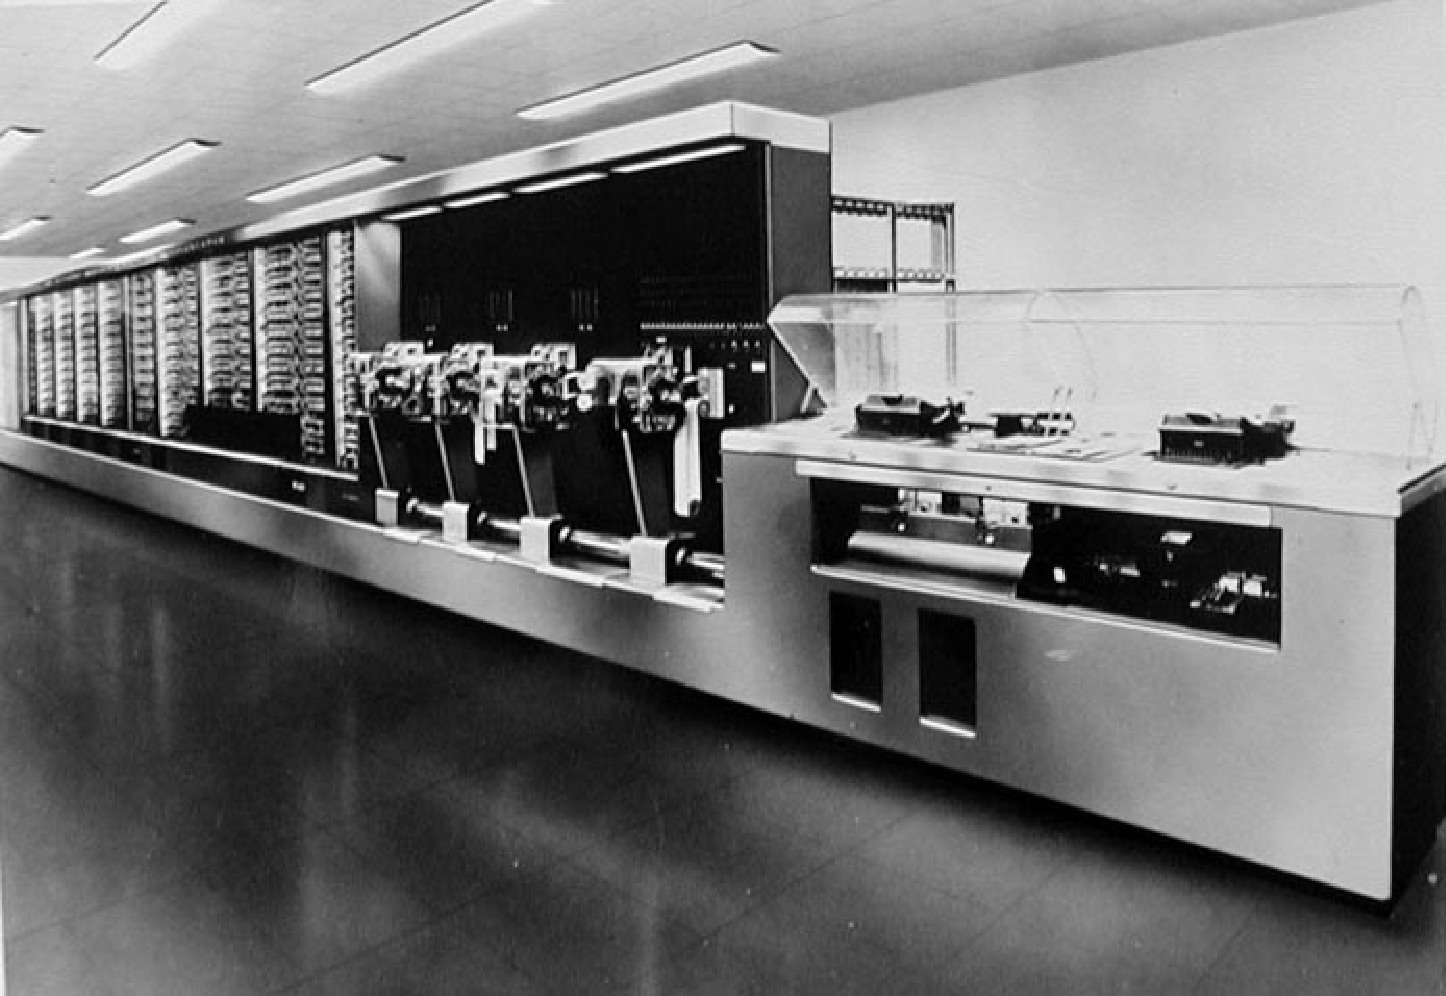
\includegraphics{ch0/fig04.pdf}}
\caption{Máy tính Mark I}
  \label{fig:fig0.4}
\end{figure}


Từ đó đến nay, lịch sử của máy tính gắn liền với việc phát triển công nghệ, bao gồm việc
phát minh ra transitors và sau đó là sự phát triển của các mạch tích hợp, sự xuất hiện
truyền thông qua vệ tinh, và tiến bộ trong công nghệ quang. Ngày nay, một chiếc máy tính
nhỏ cầm tay có thể có hiệu suất tính toán lớn hơn so với máy tính kích thước bằng cả căn
phòng của những năm 1940 và có thể trao đổi thông tin nhanh chóng qua qua hệ thống truyền
thông toàn cầu.

Một bước quan trọng làm cho máy tính trở nên phổ biến là sự phát triển của máy tính để
bàn~(desktop computer).  Những máy này bắt nguồn từ những người ưa thích máy tính, họ bắt
đầu thử tự làm các máy tính tại nhà ngay sau khi có những chiếc máy tính dùng trong nghiên
cứu vào những năm 1940. Cũng chính vì ham thích, Steve Jobs và Stephen Wozniak đã tạo ra
chiếc máy tính dùng ở nhà có thể thương mại được, và đến năm 1976, họ đã thành lập Apple
Computer, Inc, để sản xuất và bán các sản phẩm của họ. Các công ty khác cũng có các sản
phẩm tương tự trên thị trường là Commodore, Heathkit, và Radio shack. Mặc dù các sản phẩm
này rất được những người yêu thích máy tính ưa chuộng, chúng lại không được giới doanh
nhân chấp nhận. Và chính những doanh nhân này đã tìm đến công ty IBM để sản xuất đại trà
phục vụ nhu cầu tính toán của họ.

Năm 1981, IBM giới thiệu chiếc máy tính để bàn đầu tiên, nó được gọi là máy tính cá nhân
hay máy PC (Personal Computer). Các phần mềm cơ bản bên trong nó được phát triển bởi một
công ty mới thành lập là Microsoft. Máy PC đã thành công một cách nhanh chóng và được thừa
nhận rộng rãi trong giới doanh nhân. Ngày nay, thuật ngữ PC được sử dụng rộng rãi để chỉ
tất cả những máy (từ nhiều nhà sản xuất khác nhau) được phát triển từ máy tính để bàn của
IBM và hầu hết trong số chúng được bán kèm với các phần mềm của Microsoft. Tuy nhiên, đôi
khi thuật ngữ PC cũng được dùng chung cho cả \textit{máy tính để bàn (desktops)} hoặc
\textit{máy tính xách tay~(laptops)}.

Việc thu nhỏ kích thước của máy tính và các phát triển các tính năng của chúng đã đưa
ngành công nghệ máy tính trở thành ngành công nghệ đi đầu trong xã hội. Ngày nay, công
nghệ máy tính trở nên phổ biến đến mức việc trang bị các kiến thức về nó đã trở thành một
yêu cầu tối thiểu để hoà nhập với xã hội hiện đại. Máy tính gia đình đang được tích hợp
với các hệ thống truyền thông và giải trí. Các máy điện thoại di động và máy ảnh kỹ thuật
số bây giờ được kết hợp lại trong một thiết bị cầm tay được gọi là PDA (Personal Digital
Assistants).

Trên phạm vi rộng, công nghệ máy tính làm đã thay đổi cách điều hành của chính phủ, đã có
những tác động rất lớn đến nền kinh tế toàn cầu, dẫn đến những tiến bộ lớn lao trong
nghiên cứu khoa học. Ta khó có thể tưởng tượng được điều gì sẽ đến trong tương lai.


%%% Local Variables: 
%%% mode: latex
%%% TeX-master: "../tindaicuong"
%%% End: 

\section{Khoa học thuật toán}
Thuở ban đầu, do khả năng lưu trữ thông tin bị giới hạn và các thủ tục lập trình dài dòng,
rắc rối nên các thuật toán được sử dụng trong các máy tính toán còn rất đơn giản. Theo
thời gian, các rào cản này dần bị phá bỏ; các máy đã được ứng dụng cho các nhiệm vụ lớn
hơn và phức tạp hơn. Việc biểu diễn các nhiệm vụ phức tạp này dưới dạng thuật toán đã bắt
đầu thách thức khả năng của con người. Chính vì vậy, ngày càng có nhiều nghiên cứu hướng
về thuật toán và lập trình.

Trong bối cảnh này, các kết quả lý thuyết của các nhà toán học mới bắt
đầu mới thể hiện tầm quan trọng của nó. Nhờ định lý về tính không toàn
vẹn của G\"odel, các nhà toán học đã bắt đầu nghiên cứu các vấn đề
liên quan đến thuật toán nảy sinh từ công nghệ cao. Từ đây, nổi lên
một nghành khoa học mới, gọi là \textit{khoa học máy tính}.

Ngày nay, khoa học máy tính cũng được coi như là như là khoa học thuật
toán. Phạm vi của ngành khoa học này rất rộng, liên quan đến cả toán
học, kỹ thuật, tâm lý học, sinh học, quản trị kinh doanh, và ngôn ngữ
học. Trong các chương tiếp theo, ta sẽ thảo luận nhiều vấn đề
khác nhau của ngành khoa học này. Với mỗi vấn đề, mục tiêu của chúng
ta bao gồm: giới thiệu các ý tưởng trung tâm, các vấn đề đang được
nghiên cứu, và một vài phương pháp đang được sử dụng để phát triển tri
thức trong lĩnh vực này.

Để có được một bức tranh tổng thể về khoa học máy tính, ta xem
xét những câu hỏi sau đây:

\begin{figure}[tb] 
\centering
    \scalebox{0.4}{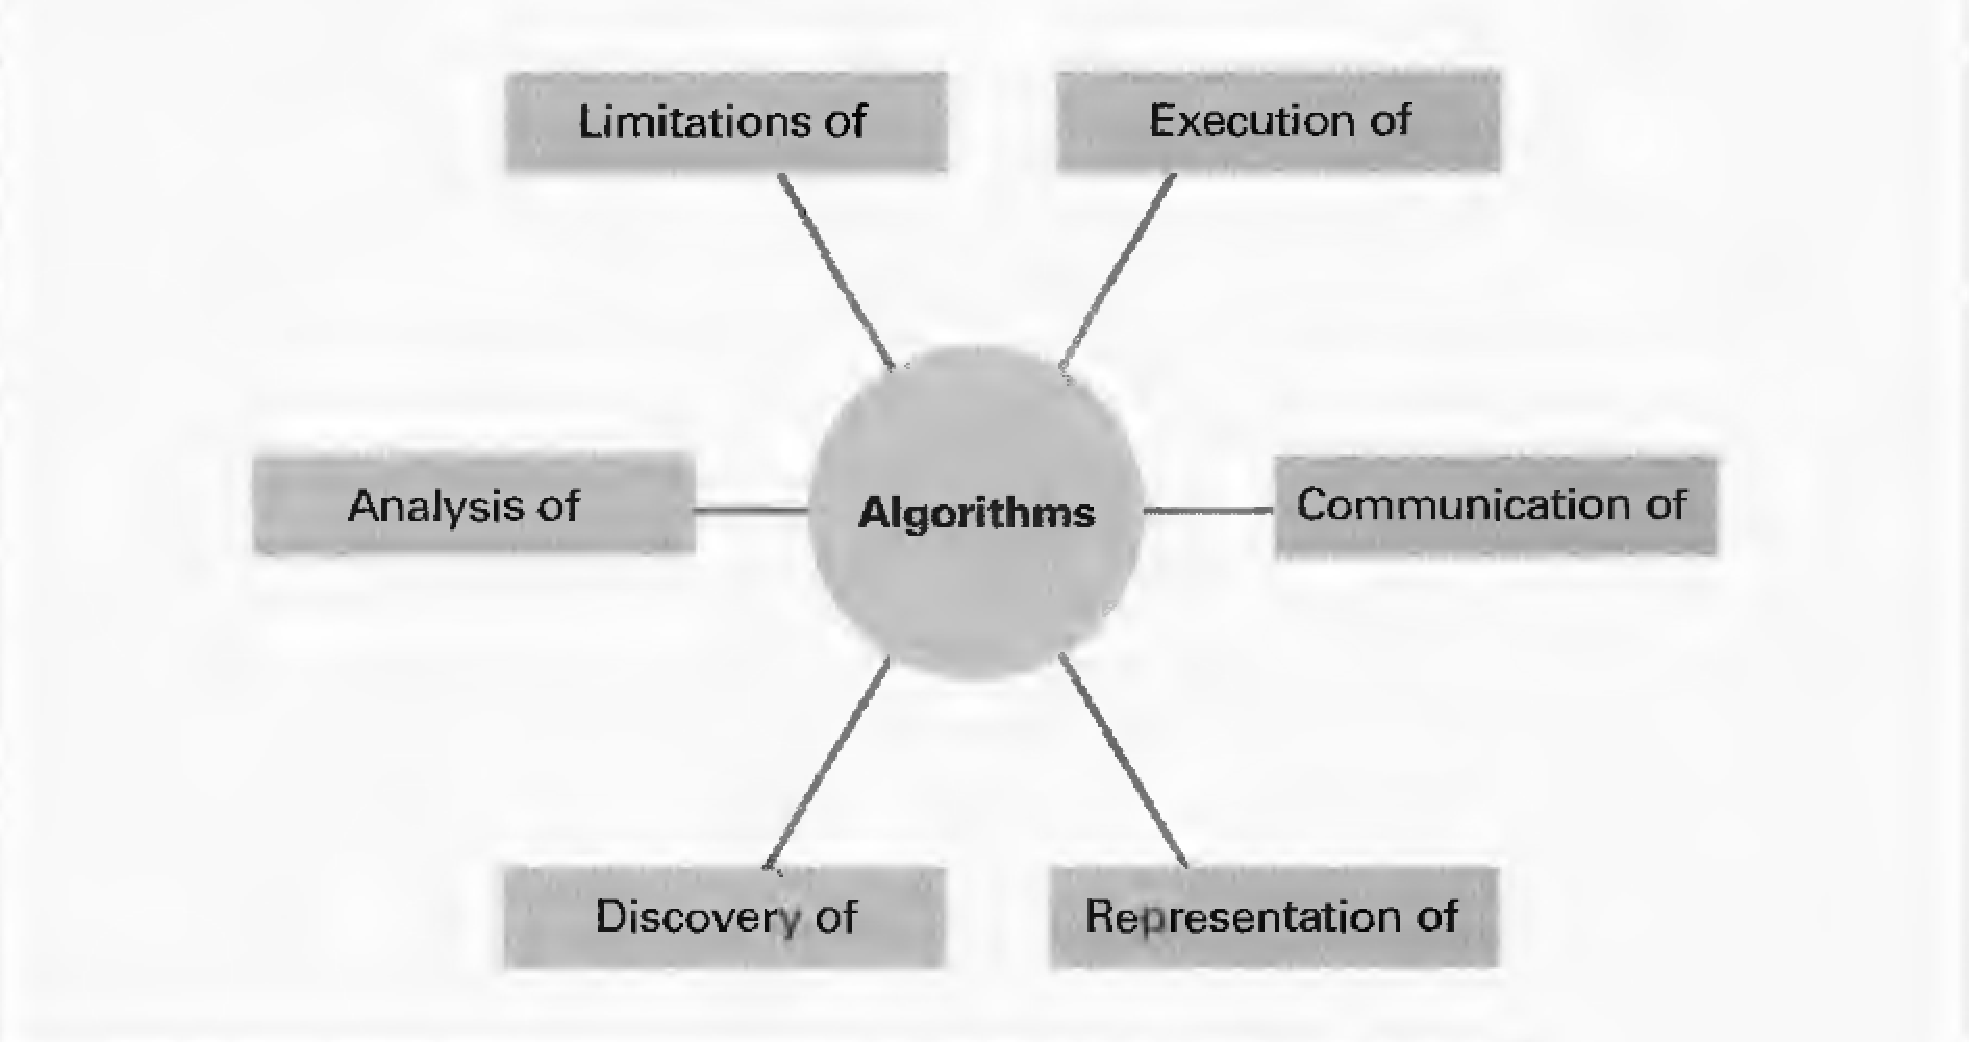
\includegraphics{ch0/fig05.pdf}}
\caption{Vai trò trung tâm của thuật toán trong khoa học máy tính}
  \label{fig:fig0.5}
\end{figure}

\begin{itemize}
\item Những bài toán nào có thể được giải bằng thuật toán?

\item Làm sao để có thể phát hiện ra thuật toán một cách dễ dàng hơn?

\item Làm sao để biểu diễn và truyền tải thuật toán một cách tốt
  hơn?

\item Làm sao để các kiến thức về thuật toán giúp ta tạo ra
  các máy tốt hơn?

\item Làm sao để có thể phân tích và so sánh các đặc trưng 
  của các thuật toán khác nhau?
\end{itemize}

Chú ý rằng các câu hỏi này đều hướng đến một chủ đề chung là nghiên
cứu thuật toán~(Hình~\ref{fig:fig0.5})




%%% Local Variables: 
%%% mode: latex
%%% TeX-master: "../tindaicuong"
%%% End: 

\section{Khái niệm trừu tượng}
 
Bởi vì khái niệm trừu tượng được sử dụng rất nhiều trong khoa học máy tính và thiết kế hệ
thống máy tính nên ta cần phải hiểu khái niệm đó ngay từ trong chương mở đầu này. Thuật
ngữ \textbf{trừu tượng}~(abstraction) ở đây nhằm chỉ sự phân biệt giữa tính chất bên ngoài
của một đối tượng và chi tiết hình thành bên trong của đối tượng đó. Nhờ trừu tượng mà ta
có thể bỏ qua chi tiết bên trong của các thiết bị phức tạp như máy tính, ô-tô, hoặc lò
vi-ba sóng; thay vào đó chỉ cần nắm bắt được các giao diện chức năng để sử dụng.  Hơn nữa,
nhờ công cụ trừu tượng nên người ta mới xây dựng được những hệ thống phức tạp.  Máy tính,
ôtô, và các lò vi-ba sóng được tạo nên từ các thành phần, mỗi thành phần lại được xây dựng
từ các thành phần nhỏ hơn. Mỗi thành phần biểu diễn một mức trừu tượng. Ở mỗi mức trừu
tượng, ta sử dụng lại các thành phần mức thấp hơn mà không phải quan tâm chi tiết xem
chúng hình thành thế nào.

Nhờ có trừu tượng, ta có thể xây dựng, phân tích, và quản lý các hệ thống máy tính lớn,
phức tạp. Các hệ thống này rất rắc rối nếu nhìn các đối tượng của chúng một cách chi
tiết. Theo từng mức trừu tượng, ta chỉ nhìn hệ thống dưới dạng các thành phần, gọi là các
\textbf{công cụ trừu tượng} (abstract tools), mà bỏ qua chi tiết về cấu thành bên trong
của chúng. Điều này cho phép ta tập trung xem xét xem các thành phần (ở cùng mức) tương
tác với nhau như thế nào và làm thế nào để tập hợp chúng lại thành một thành phần ở mức
cao hơn. Bởi vậy, ta có thể hiểu từng phần của hệ thống.

Ta nhấn mạnh rằng việc trừu tượng không chỉ giới hạn trong phạm vi khoa học và công
nghệ. Nó là kỹ thuật đơn giản hoá quan trọng tạo ra lối sống của xã hội. Rất ít người
trong chúng ta hiểu sự tiện lợi trong cuộc hàng ngày được thực hiện như thế nào-- ta ăn và
mặc những thứ mà bản thân ta không thể làm ra được, ta sử dụng các thiết bị điện mà không
cần phải hiểu về công nghệ chế tạo ra nó. Ta sử dụng các dịch vụ của những người khác mà
không cần biết một cách chi tiết về nghề của họ. Từng bước, người ta cố gắng chuyên biệt
cách thực hiện một số thứ trong xã hội, còn những người khác chỉ cần cố gắng tìm hiểu để
sử dụng các kết quả đó như là công cụ trừu tượng. Theo cách này, kho các công cụ trừu
tượng của xã hội được mở rộng, và khả năng của xã hội không ngừng tiến xa hơn.

Ta còn gặp lại chủ đề trừu tượng nhiều lần trong nghiên cứu. Ta sẽ thấy rằng các thiết bị
máy tính được xây dựng ở mức của các công cụ trừu tượng.  Sự phát triển của các hệ thống
phần mềm lớn là theo cách mô đun hoá trong đó mỗi mô đun được sử dụng như là một công cụ
trừu tượng trong mô đun lớn hơn. Hơn nữa, trừu tượng đóng vai trò quan trọng trong nhiệm
vụ phát triển ngành khoa học máy tính, cho phép các các nhà nghiên cứu hướng sự chú ý tới
các lĩnh vực đặc biệt bên trong một lĩnh vực phức tạp. Trên thực tế, cách tổ chức của cuốn
sách này phản ánh đặc trưng của khoa học. Mỗi chương trọng tâm vào một chủ đề cụ thể,
chương này độc lập với chương khác, nhưng khi ghép lại cùng nhau nó trở thành một tài liệu
tổng quan dễ hiểu về các lĩnh vực rộng được nghiên cứu.

%%% Local Variables: 
%%% mode: latex
%%% TeX-master: "../tindaicuong"
%%% End: 

  
%%% Local Variables: 
%%% mode: latex
%%% TeX-master: "../tindaicuong"
%%% End: 
